\documentclass[15pt]{beamer}
\usetheme{Boadilla}
\usepackage{tikz}
\usepackage{graphicx}
\usepackage{amsmath}
\usetikzlibrary{shapes.geometric,arrows, positioning, fit}

\title{Presentation Arrowhead framework}
\author{}
\institute{Luleå University of Technology}
\date{\today}

\begin{document}
\begin{frame}
    \titlepage
\end{frame}

\begin{frame}
    \frametitle{Overview}
    \tableofcontents
\end{frame}

\section{Core systems}
    \subsection{Service Registry}
    \subsection{Orchestrator}
    \subsection{Authorization system}
    \begin{frame}
    \frametitle{Core systems}
    Three mandatory core systems and services
        \begin{itemize}
            \item Service Registry
            \item Orchestrator
            \item Authorization system
        \end{itemize}
    In our implementation of the Arrowhead framework we will use the following terminology
        \begin{itemize}
            \item Consumer
                \begin{itemize}
                    \item Gets data from provider and processes that data i.e. logging, calling other functions.
                \end{itemize}
            \item Provider
                \begin{itemize}
                    \item Collects data from sensors, databases or other applications and sends that data to the consumer.
                \end{itemize}
        \end{itemize}
\end{frame}
    
\section{Service Registry}
    \begin{frame}
    \frametitle{Service Registry}
    Implements three methods
    \begin{itemize}
        \item Register 
            \begin{itemize}
                \item  adds a new service to the the service registry 
                \item  contains metadata about endpoint, i.e. name, IP address and port etc.
            \end{itemize}
        \item Unregister
            \begin{itemize}
                \item  removes a service from the the service registry 
            \end{itemize}
        \item Query
            \begin{itemize}
                \item  Translates system name into information about the physical endpoint i.e. IP address and port
            \end{itemize}
    \end{itemize}
\end{frame}
    
\section{Authorization system}
    \begin{frame}  
    \frametitle{Authorization system}
    
    Implements two methods
    
    \begin{itemize}
        \item Authorization control
        \begin{itemize}
            \item Sets up rules for which services are allowed to access each other.
            \item Specifies which protocols will be used for communication.
            \item Sets up rules for communication within local cloud, also called intracloud authorization.
            \item Sets up rules for communication with remote clouds, also called intercloud authorization.
        \end{itemize}
        \item Token generation
            \begin{itemize}
                \item Generates a token used for accessing services within cloud, currently only supported between remote clouds. 
                \item Will not be used in our implementation, we will use certificates.
            \end{itemize}
            
    \end{itemize}
    
\end{frame}
    
\section{Orchestrator}
    \begin{frame}  
    \frametitle{Orchestrator}
    Implements two methods
    \begin{itemize}
        \item Orchestration pull
            \begin{itemize}
                \item An Application system requests requests a service.
                \item If the requesting application system is allowed to access requested service the 
                      physical endpoints are returned.
                \item If the requesting application system is not allowed to access requested service or the        service doesn't exist an error code will be returned.
            \end{itemize}
        \item Orchestration push
        \begin{itemize}
            \item The Orchestrator pushes new information on Application Systems, with information about physical endpoints and which services that are connected.
            \item Only required for store orchestration.
        \end{itemize}
        
    \end{itemize}

\end{frame}

\begin{frame}
    \frametitle{Orchestrator}
    Two types of orchestration 
    \begin{itemize}
        \item Dynamic orchestration
        \begin{itemize}
            \item Uses the application system name and authorization properties to find the appropriate providers. 
        \end{itemize}
        
        \item Store orchestration
        \begin{itemize}
            \item Uses the application system's id to query the orchestration store database for an appropriate provider. 
        \end{itemize}
    \end{itemize}

\end{frame}
    
\section{Sequence diagram}
    \begin{frame}
    \frametitle{Sequence diagram}
    \begin{figure}
        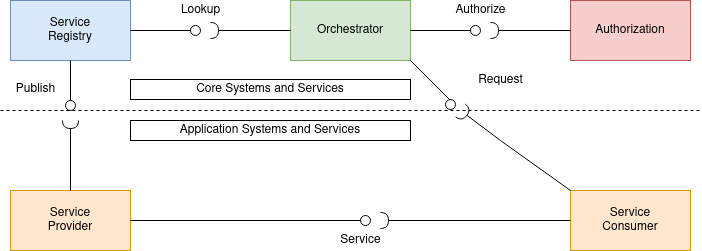
\includegraphics[width=\textwidth]{frames/images/Untitled Diagram.png}
        \end{figure}
\end{frame}
    
\section{Implementation}
    \begin{frame}
    \frametitle{Implementation}
    \begin{itemize}
        \item MySQL database
        \item Swagger UI
        \item Python and ROS client
    \end{itemize}
    
\end{frame}
    
\section{Advantages and purpose}
    \begin{frame}
    \frametitle{Advantages and purpose}
    \begin{itemize}
        \item Main advantage of using Arrowhead framework is security
            \begin{itemize}
                \item IoT applications are well known for their lack of security.
                \item Arrowhead framework is a way to solve some of those security issues.
            \end{itemize}
        \item Our first purpose is to test if it is possible to use Arrowhead in a secure way.
        \item Our second purpose is to provide an API for integration Arrowhead framework, python and ROS for secure embedded systems.
    \end{itemize}
\end{frame}
    
\begin{frame}
    \begin{center}
        \Huge Questions?
    \end{center}
\end{frame}

\end{document}
